\chapter{The LEGEND experiment}
\label{ch:legend}

The Large Enriched Germanium Experiment for Neutrinoless double beta Decay (LEGEND) is a next-generation experimental program searching for the $0\nu\beta\beta$ decay of ${}^{76}$Ge. Located deep underground at the Gran Sasso National Laboratories (LNGS) in Italy, under a rock overburden of approximately 3500 m.w.e. (meter water equivalent), LEGEND operates in an environment heavily shielded from cosmic radiation.

The experiment is designed to operate in two distinct phases. In its first stage, LEGEND-200, it is currently operating with roughly 200 kg of enriched germanium detectors. Its objective is to achieve a background index of $2 \times 10^{-4}$ cts/(keV$\cdot$kg$\cdot$yr) to reach a discovery sensitivity greater than $10^{27}$ yr with 1 t$\cdot$yr of exposure. The subsequent phase, LEGEND-1000, will scale the target mass up to 1000 kg, aiming for an unprecedented background goal of $1 \times 10^{-5}$ cts/(keV$\cdot$kg$\cdot$yr) to reach a sensitivity greater than $10^{28}$ yr with an exposure of 10 t$\cdot$yr.

To achieve such ambitious goals, LEGEND builds upon the successful technologies and background mitigation strategies developed by its predecessors, the GERDA and \textsc{Majorana Demonstrator} experiments. By utilizing High-Purity Germanium (HPGe) detectors enriched in ${}^{76}$Ge, the experiment benefits from the ``source-equals-detector'' approach. This maximizes the detection efficiency and exploits the outstanding energy resolution of semiconductor detectors to clearly separate the mono-energetic $0\nu\beta\beta$ signal from the $2\nu\beta\beta$ irreducible continuous background.

Reaching the required ultra-low background regime demands a multi-layered active and passive shielding strategy. This is accomplished by operating the bare germanium array directly in an instrumented Liquid Argon (LAr) cryostat, surrounded by a large water Cherenkov veto, and by employing sophisticated signal processing techniques to reject localized background events. The following sections detail the experimental apparatus and the event selection methods crucial to the experiment's success. \cite{LEGEND:GeDet}

\section{Experimental setup}
\label{sec:expsetup}
The experimental setup of the LEGEND program builds upon the decommissioned GERDA experiment. It repurposes GERDA infrastructure and inherits its shielding concept, which relies on a low-Z shield (water and argon) and an active veto system based on the detection of argon scintillation light. \cite{LEGEND:introSetup}

The whole structure of the setup is shown in Figure~\ref{fig:L200setup} and consists of:
\begin{itemize}
    \item 200 kg of hyper pure Germanium detectors (HPGe);
    \item a liquid Argon (LAr) cryostat;
    \item a water tank for Cherenkov light detection.
\end{itemize}

\begin{figure}[H]
    \centering
    % Immagine a sinistra
    \begin{minipage}{0.48\textwidth}
        \centering
        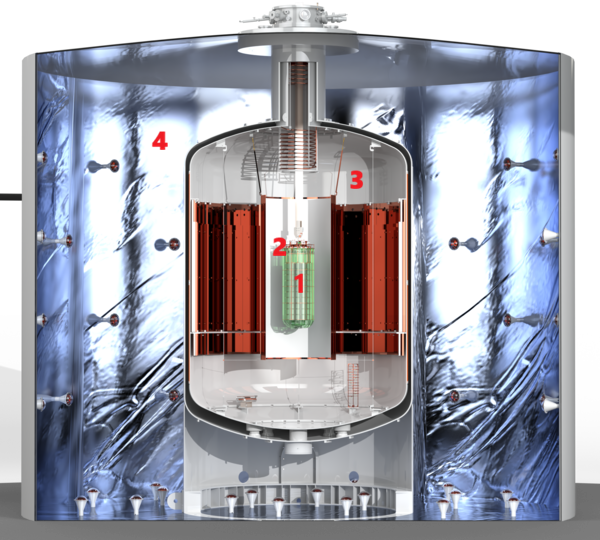
\includegraphics[width=\linewidth]{figures/LEGENDwholeSetup_con.numeri.png}
    \end{minipage}\hfill
    % Immagine a destra
    \begin{minipage}{0.28\textwidth}
        \centering
        % SOSTITUISCI IL NOME DEL FILE QUI SOTTO
        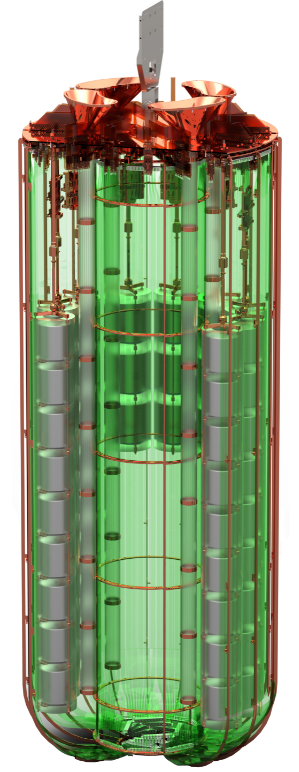
\includegraphics[width=\linewidth]{figures/LEGENDLAr.png}
    \end{minipage}
    
    \caption{On the left the whole experimental setup for the LEGEND-200 phase: the picture shows the HPGe detectors (1), the LAr instrumentation (2), the LAr cryostat (3) and the water tank provided with the Cherenkov detectors (4). On the right a closeup of the LAr instrumentation where the detector strings are visible. Taken from \cite{LEGEND:setup}}
    \label{fig:L200setup}
\end{figure}

\paragraph{Germanium detectors}
The High Purity Germanium (HPGe) detectors are semiconductor diodes sensitive to ionizing radiation and $\gamma$-rays. They provide excellent energy resolution and high detection efficiency, acting as both the source and detector for double-beta decay. 
% The HPGe detectors operate with a reverse bias voltage, which depletes almost the entire volume of free charge carriers. A high voltage (up to 5~kV) is applied to the $n^+$ electrode, which features a relatively thick ($\sim 0.7$~mm) Li-diffused dead layer, while the signal is readout from the thin ($\sim 0.3$~$\mu$m) $p^+$ electrode, created via boron implantation.

LEGEND-200 utilizes p-type germanium detectors from previous experiments, including Broad Energy Germanium (BEGe) and semi-Coaxial (COAX) detectors from GERDA, and P-type Point Contact (PPC) detectors from the \textsc{Majorana Demonstrator}. To achieve the 200~kg array, newly developed Inverted Coaxial Point Contact (ICPC) detectors are incorporated, which make up more than 60\% of the total mass. All of them are made from isotopically enriched material in ${}^{76}$Ge up to 90\%.

These detectors are mounted on supports made of active PolyEthylene Naphthalate (PEN), a scintillating plastic material known for its ability to improve background rejection, and are arranged in 12 strings. To maintain high radiopurity near the detector array, low-mass Majorana components and underground electroformed copper are used to reduce the effects of~${}^{238}$U and~${}^{232}$Th decay chains and cosmogenic activation of~${}^{60}$Co in copper. Each HPGe string is enclosed in a TPB-coated nylon cylinder, called Nylon Mini Shroud (NMS), to minimize the LAr volume around the detectors, preventing the capture of radioactive ions like~${}^{42}$K by electric fields on the detector surfaces. \cite{LEGENDsetup-details}

The detectors and liquid argon instrumentation are assembled in the clean room above the cryostat in a glove box which is flushed with nitrogen to reduce/avoid radon deposition on the detectors and protects the insulating groove between the detector $p^+$ and $n^+$ electrodes by an inert atmosphere. The detectors are assembled into strings and, together with the liquid argon instrumentation, placed inside the lock. When the lock is closed, several pumping and purging cycles follow. \cite{LEGEND:setup}

\paragraph{Liquid Argon (LAr) cryostat}
A 4~m-diameter vacuum-insulated stainless steel cryostat with 64~m$^3$ of purified Liquid Argon (LAr) is present. The ultra-pure LAr acts as a cooling medium for the germanium detectors and an additional shield for external radiation. At the bottom of the cryostat, the LEGEND LAr Monitoring Apparatus (LLAMA) is placed, allowing to monitor the purification levels of the LAr continuously.

The center of the cryostat contains a 1374~mm-diameter and 3~m-height cylinder, made of copper-tetratex foil coated internally with TetraPhenyl Butadiene (TPB), called WaveLength-Shifting Reflector (WLSR). The WLSR is designed to separate the innermost LAr volume (about 6~t of LAr), working as further shielding for detector systems and as a reflector of the LAr scintillation light.

The LAr instrumentation is located within the WLSR and consists of two concentric WaveLength-Shifting (WLS) fiber shrouds that surround the germanium detectors (Fig. \ref{fig:L200setup} right). The WLS fibers are coupled to SiPMs at both ends. The LAr instrumentation is crucial for detecting background events that deposit energy in the LAr volume surrounding the germanium detectors. \cite{LEGENDsetup-details}

The cryogenic infrastructure of the cryostat includes the liquid argon and nitrogen storage tanks, a valve box which houses manual and remotely controlled valves for LN$_2$/LAr and a radon trap, and piping inside the cryostat. The latter includes two copper spirals as heat exchangers for the cooling of LAr with LN$_2$, a LAr filling line, a drainage pipe, temperature sensors at different positions, and several devices for the fill level measurement. The available aperture for the detectors in the neck is reduced because of these pipes and sensors such that this opening becomes the limiting cross section. For LEGEND-200, the installation has been replaced to enlarge the area for detectors and LAr instrumentation. \cite{LEGEND:setup}

\paragraph{Water tank}
A 10~m-diameter and 8~m-height tank with 590~m$^3$ of ultra-pure water shields from neutron and gamma backgrounds. It works also as a muon veto for residual cosmic muons through the detection of Cherenkov light with 66 PMTs (8” size) of type 9354KB/9350KB by ETL. In order
to protect the PMTs from the surrounding water, each PMT is housed in a stainless-steel encapsulation which is further developed from the design of the Borexino capsules. The PMTs are arranged in seven rings in the water tank. One ring of six PMTs is pointing inside the separate volume under the cryostat,  two rings of eight PMTs and 12 PMTs  respectively are placed on the bottom of the water tank looking upwards and four rings of 10 PMTs are placed on the wall, pointing horizontally towards the cryostat. \cite{GERDA-muonVeto} 

\section{Germanium detectors}

\subsection{Events topology}
Different events distinguished oj the basis of \ac{MSE} and \ac{SSE}

\section{Background suppression}
Background is the main issue in the LEGEND experiment and avery sibngle part of it has been built considering that background has to be limited as much as possible.